\chapter[Реализация модуля]{Реализация модуля автогенерации платформо-зависимых констант}
\label{sec:Chapter3} \index{Chapter3}

\section{Описание основной идеи решения}
В дальнейшем для определённости предполагается, что исходный код виртуальной машины собирается с помощью утилиты CMake \cite{cmake}.
Данная утилита поддерживает кросс-сборки, позволяя выбрать не только архитектуру микропроцессора, но также уточнить операционную систему целевого устройства (или её отсутствие).
Это позволяет генерировать образы программ под большое множество устройств.
В случае виртуальной машины, подготовив на сервере соответствующий образ и загрузив его на телефон, получается корректно работающая виртуальная машина, способная исполнять байткод, каким-либо образом попадающий на устройство в дальнейшем, а также имеющая JIT- и AOT-компилятор (рис. \ref{fig:device_image}).

\begin{figure}[H]
    \centering
    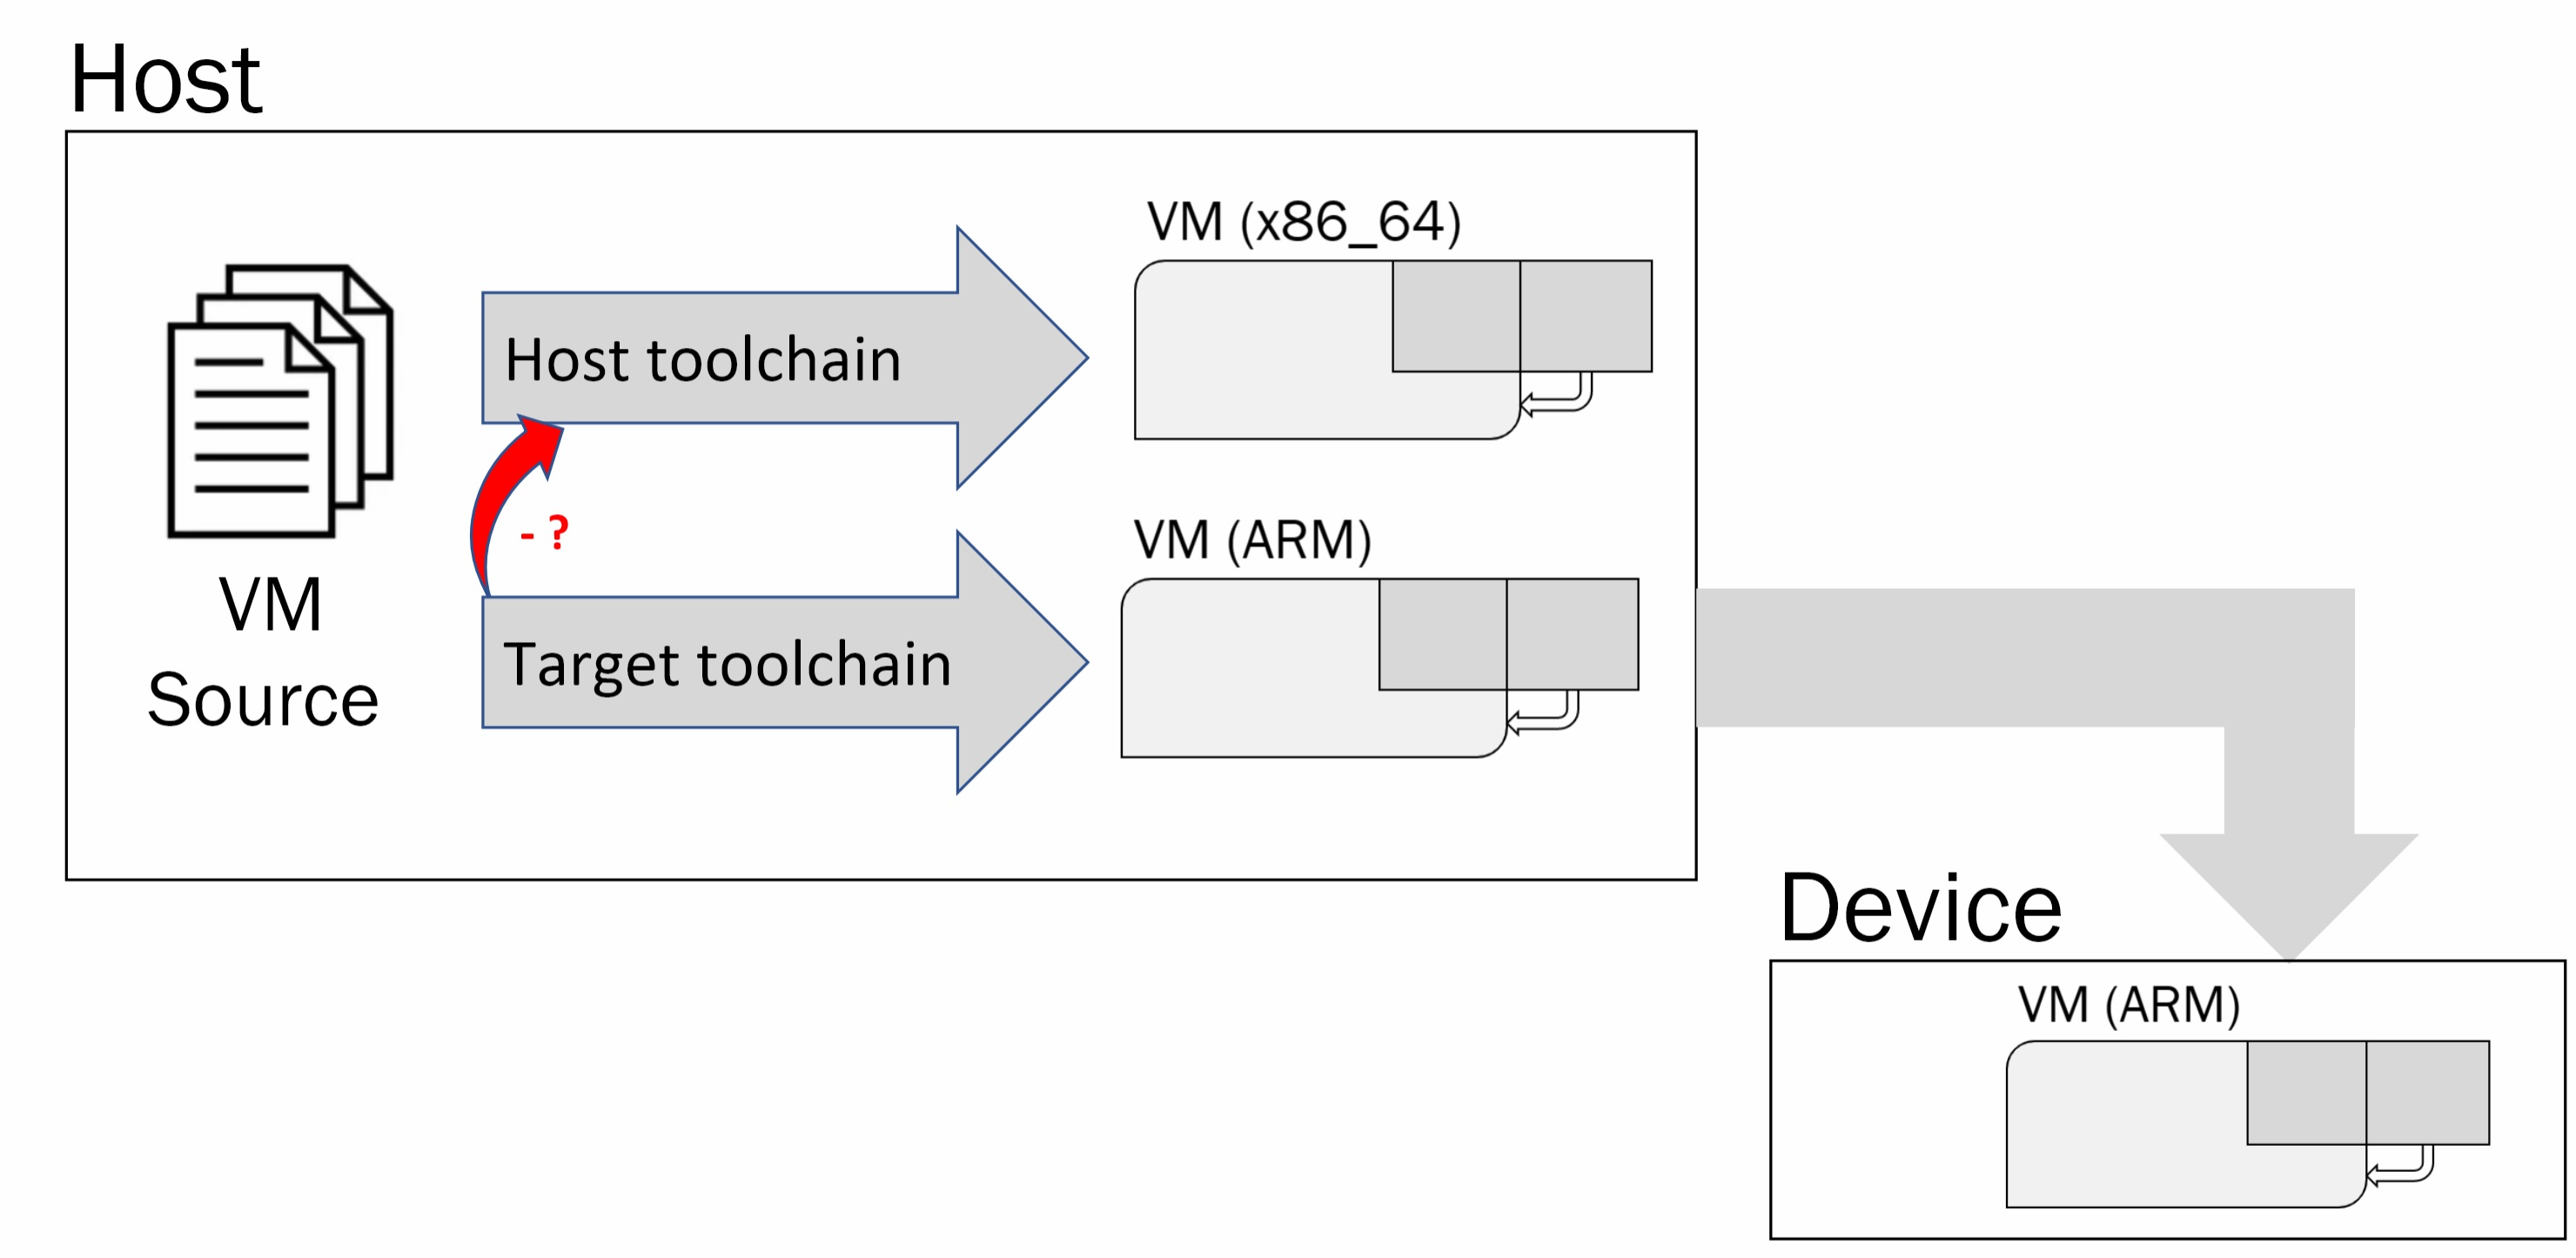
\includegraphics[scale=0.3]{device_image.jpg}
    \caption{Процесс появления виртуальной машины на таргет-устройстве. Под красной стрелкой можно понимать проблему вычисления гостевых констант.}
    \label{fig:device_image}
\end{figure}

Чтобы иметь возможность подготавливать AOT-файлы для телефона на сервере (мотивация чего описана в Главе \ref{sec:Chapter0}), можно каким-либо образом извлечь значения гостевых констант из процесса сборки образа для гостевого устройства и добавить их в некотором виде в исходный код хост-сборки AOT-компилятора.
Идея компактной <<псевдо-сборки>>, которая не полностью подготавливает образ виртуальной машины, а служит лишь для извлечения необходимой информации, и является основной идеей описываемого решения.

\section{Схема вычисления гостевых констант}
Для начала, все платформо-зависимые константы объединяются в специальную единицу трансляции, формат которой приведён на рис. \ref{fig:asm_defines}.

\begin{figure}[H]
    \centering
    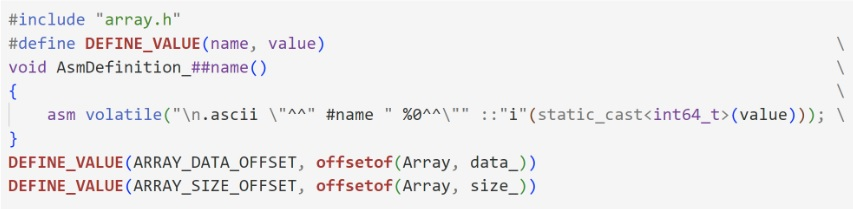
\includegraphics[scale=1.5]{asm_defines.jpg}
    \caption{Формат описываемой единицы трансляции с примером платформо-зависимых констант (смещения до полей структуры \textit{Array}).}
    \label{fig:asm_defines}
\end{figure}

\definecolor{myred}{rgb}{0.5,0,0}
\definecolor{mygr}{rgb}{0,0.5,0}
\definecolor{mygray}{rgb}{0.2,0.2,0.2}
Помимо своего основного предназначения, речь о котором пойдёт далее, она обладает важным документирующим свойством: все платформо-зависимые константы оказываются определены в общем, предназначенном для них месте, а для добавления новой константы требуется лишь добавить строчку формата \lstinline[language=c++, keywordstyle=\color{myred}, keywordstyle=\bfseries\color{myred}, basicstyle=\color{blue}, commentstyle = \ttfamily\color{mygr}, morekeywords={*, DEFINE_VALUE}, breaklines=true, backgroundcolor=\color{gray}]{DEFINE_VALUE(/* id */, /* constant expression */)}.
\par
Далее, рассмотрим подробнее процесс сборки виртуальной машины из исходного кода для хост-устройства.
На стадии CMake-конфигурации помимо основной, хост-сборки, также конфигурируется с использованием соответствующего таргет-тулчейна один или несколько вспомогательных сборок, каждая из которых находится в отдельной директории внутри корневой директории сборки (рис. \ref{fig:build_dir}).

\begin{figure}[H]
    \centering
    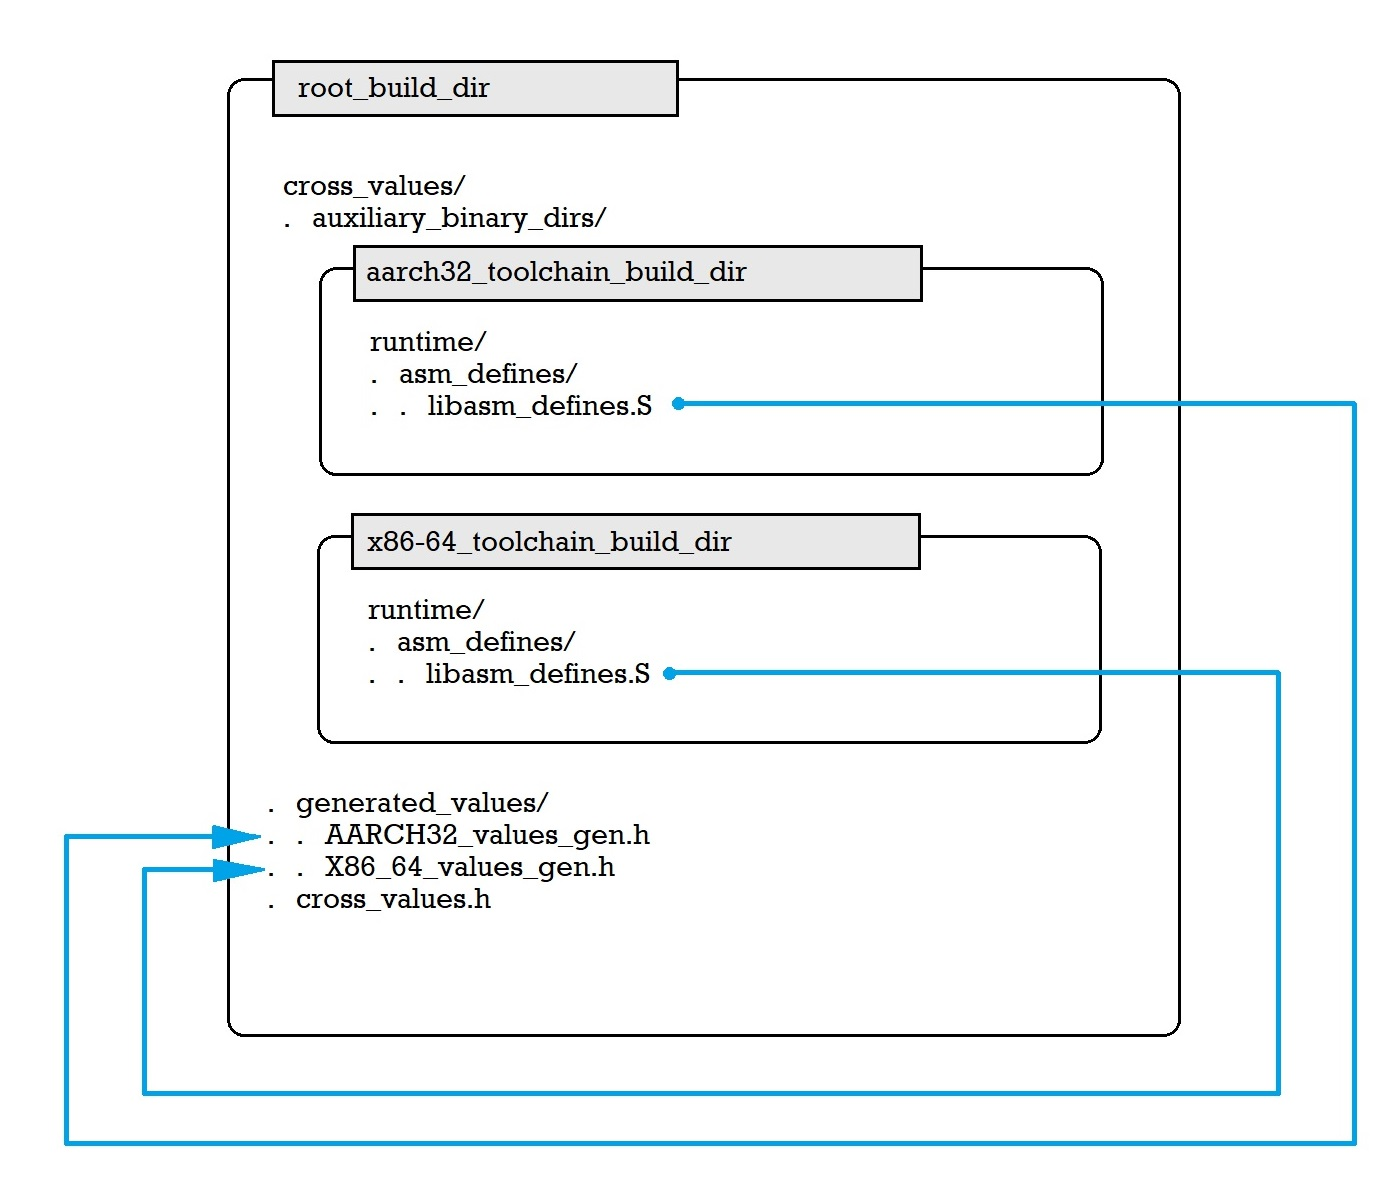
\includegraphics[scale=0.8]{build_dir.jpg}
    \caption{Схема директории сборки виртуальной машины. Голубым цветом обозначены зависимости сборки.}
    \label{fig:build_dir}
\end{figure}

Стоит отметить, что хост-платформа также может рассматриваться как одна из таргет-платформ, что показано на схеме выше.
Это позволяет унифицировать подход к выбору целевой платформы в случае поддержки AOT-компилятором виртуальной машины нескольких целевых платформ.
В каждой вспомогательной сборке, после того как она была сконфигурирована, происходит кросс-компиляция описанной выше единицы трансляции, однако не в бинарный, а ассемблерный вид. Часть такого файла изображена на рисунке \ref{fig:asm_defines_comp}.

\begin{figure}[H]
    \centering
    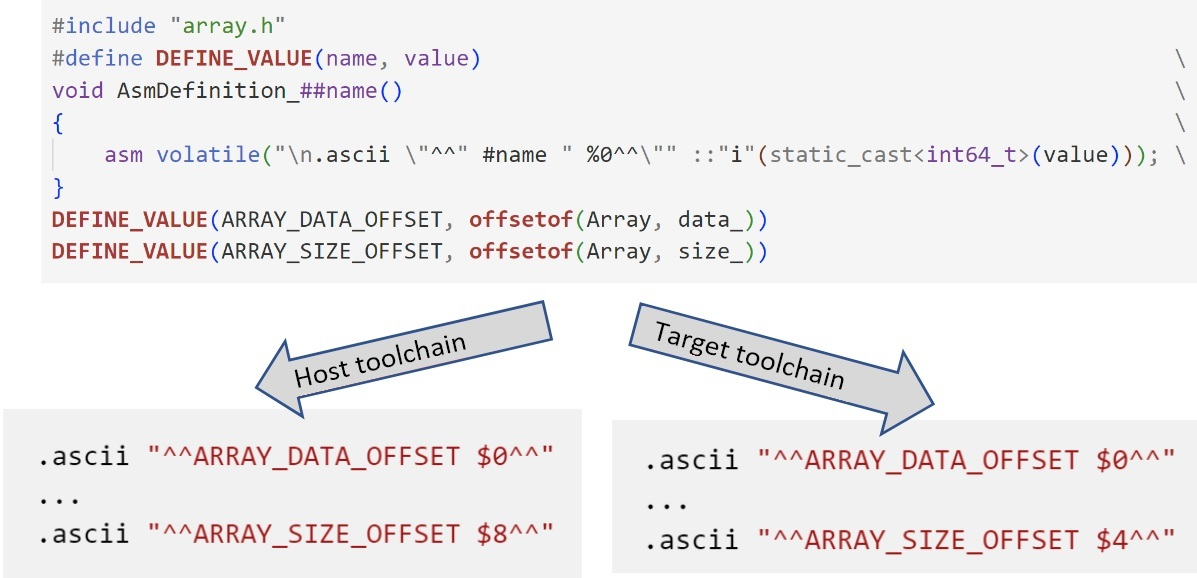
\includegraphics[scale=1]{asm_defines_comp.jpg}
    \caption{Процесс генерации ассемблерного файла с помощью таргет-тулчейнов.}
    \label{fig:asm_defines_comp}
\end{figure}

Особый формат ассемблерных вставок, в которые преобразуются макросы, соответствующие платформо-зависимым константам, позволяют достаточно просто проанализировать результат компиляции и извлечь гостевые константы в численном виде.
Полученные таким образом данные используются для определения C++-констант, имеющих одинаковые имена и разделённые пространством имён, соответствующие обозначению целевой платформы. Они оформляются в виде заголовочных файлов, которые уже могут встраиваться в платформо-специфичный код виртуальной машины, предоставляя тем самым доступ к платформо-зависимым константам (рис. \ref{fig:asm_defines_gen}).

\begin{figure}[H]
    \centering
    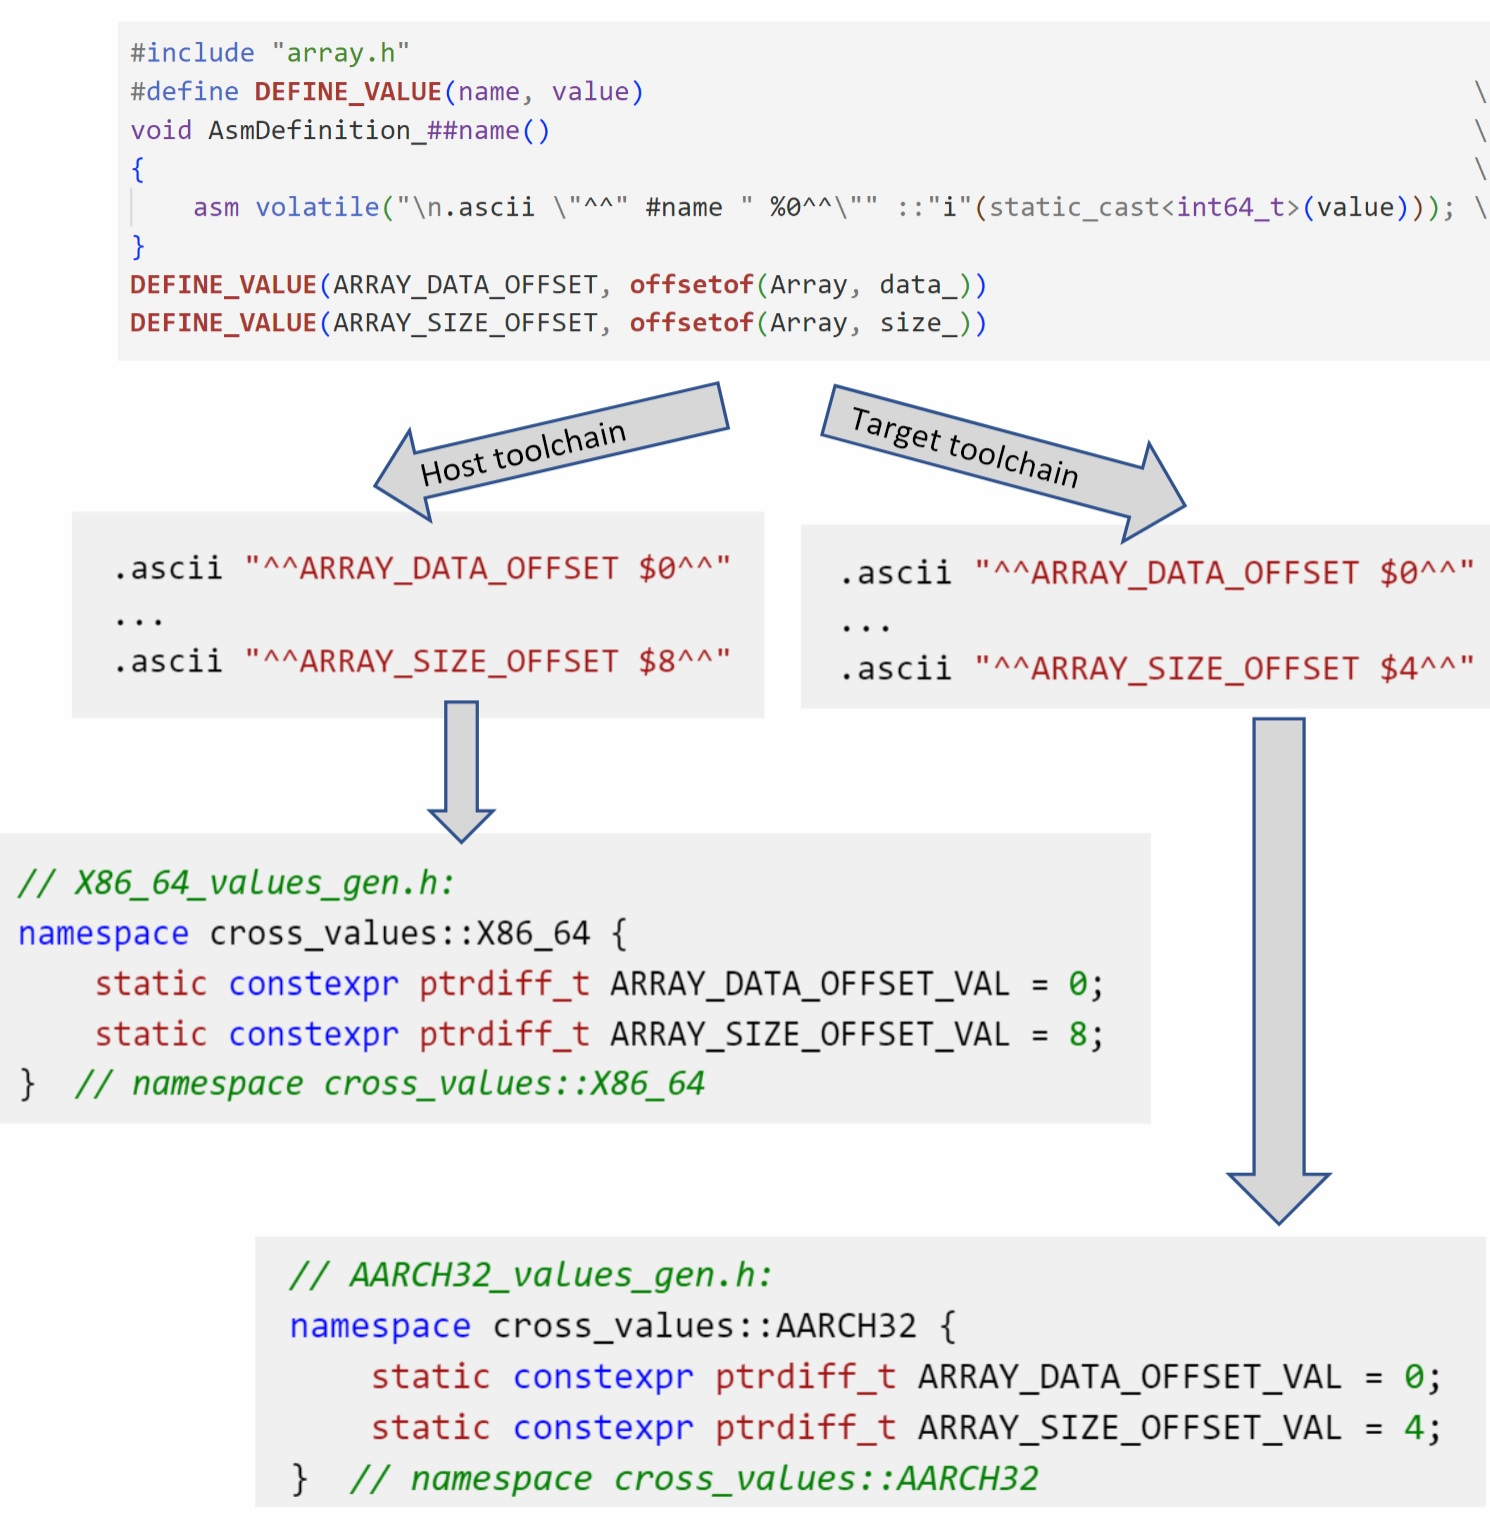
\includegraphics[scale=0.8]{asm_defines_gen.jpg}
    \caption{Схема генерации файлов, содержащих определения констант.}
    \label{fig:asm_defines_gen}
\end{figure}

После того как последний заголовочный файл сгенерирован, необходимо объединить их в один для удобства, а также сгенерировать для каждой платформо-зависимой константы геттер-функцию, позволяющую различать значения каждой из констант, принимаемые ими на целевых платформах, по некоторой переменной перечисляемого типа (рис. \ref{fig:asm_defines_getters}).

\begin{figure}[H]
    \centering
    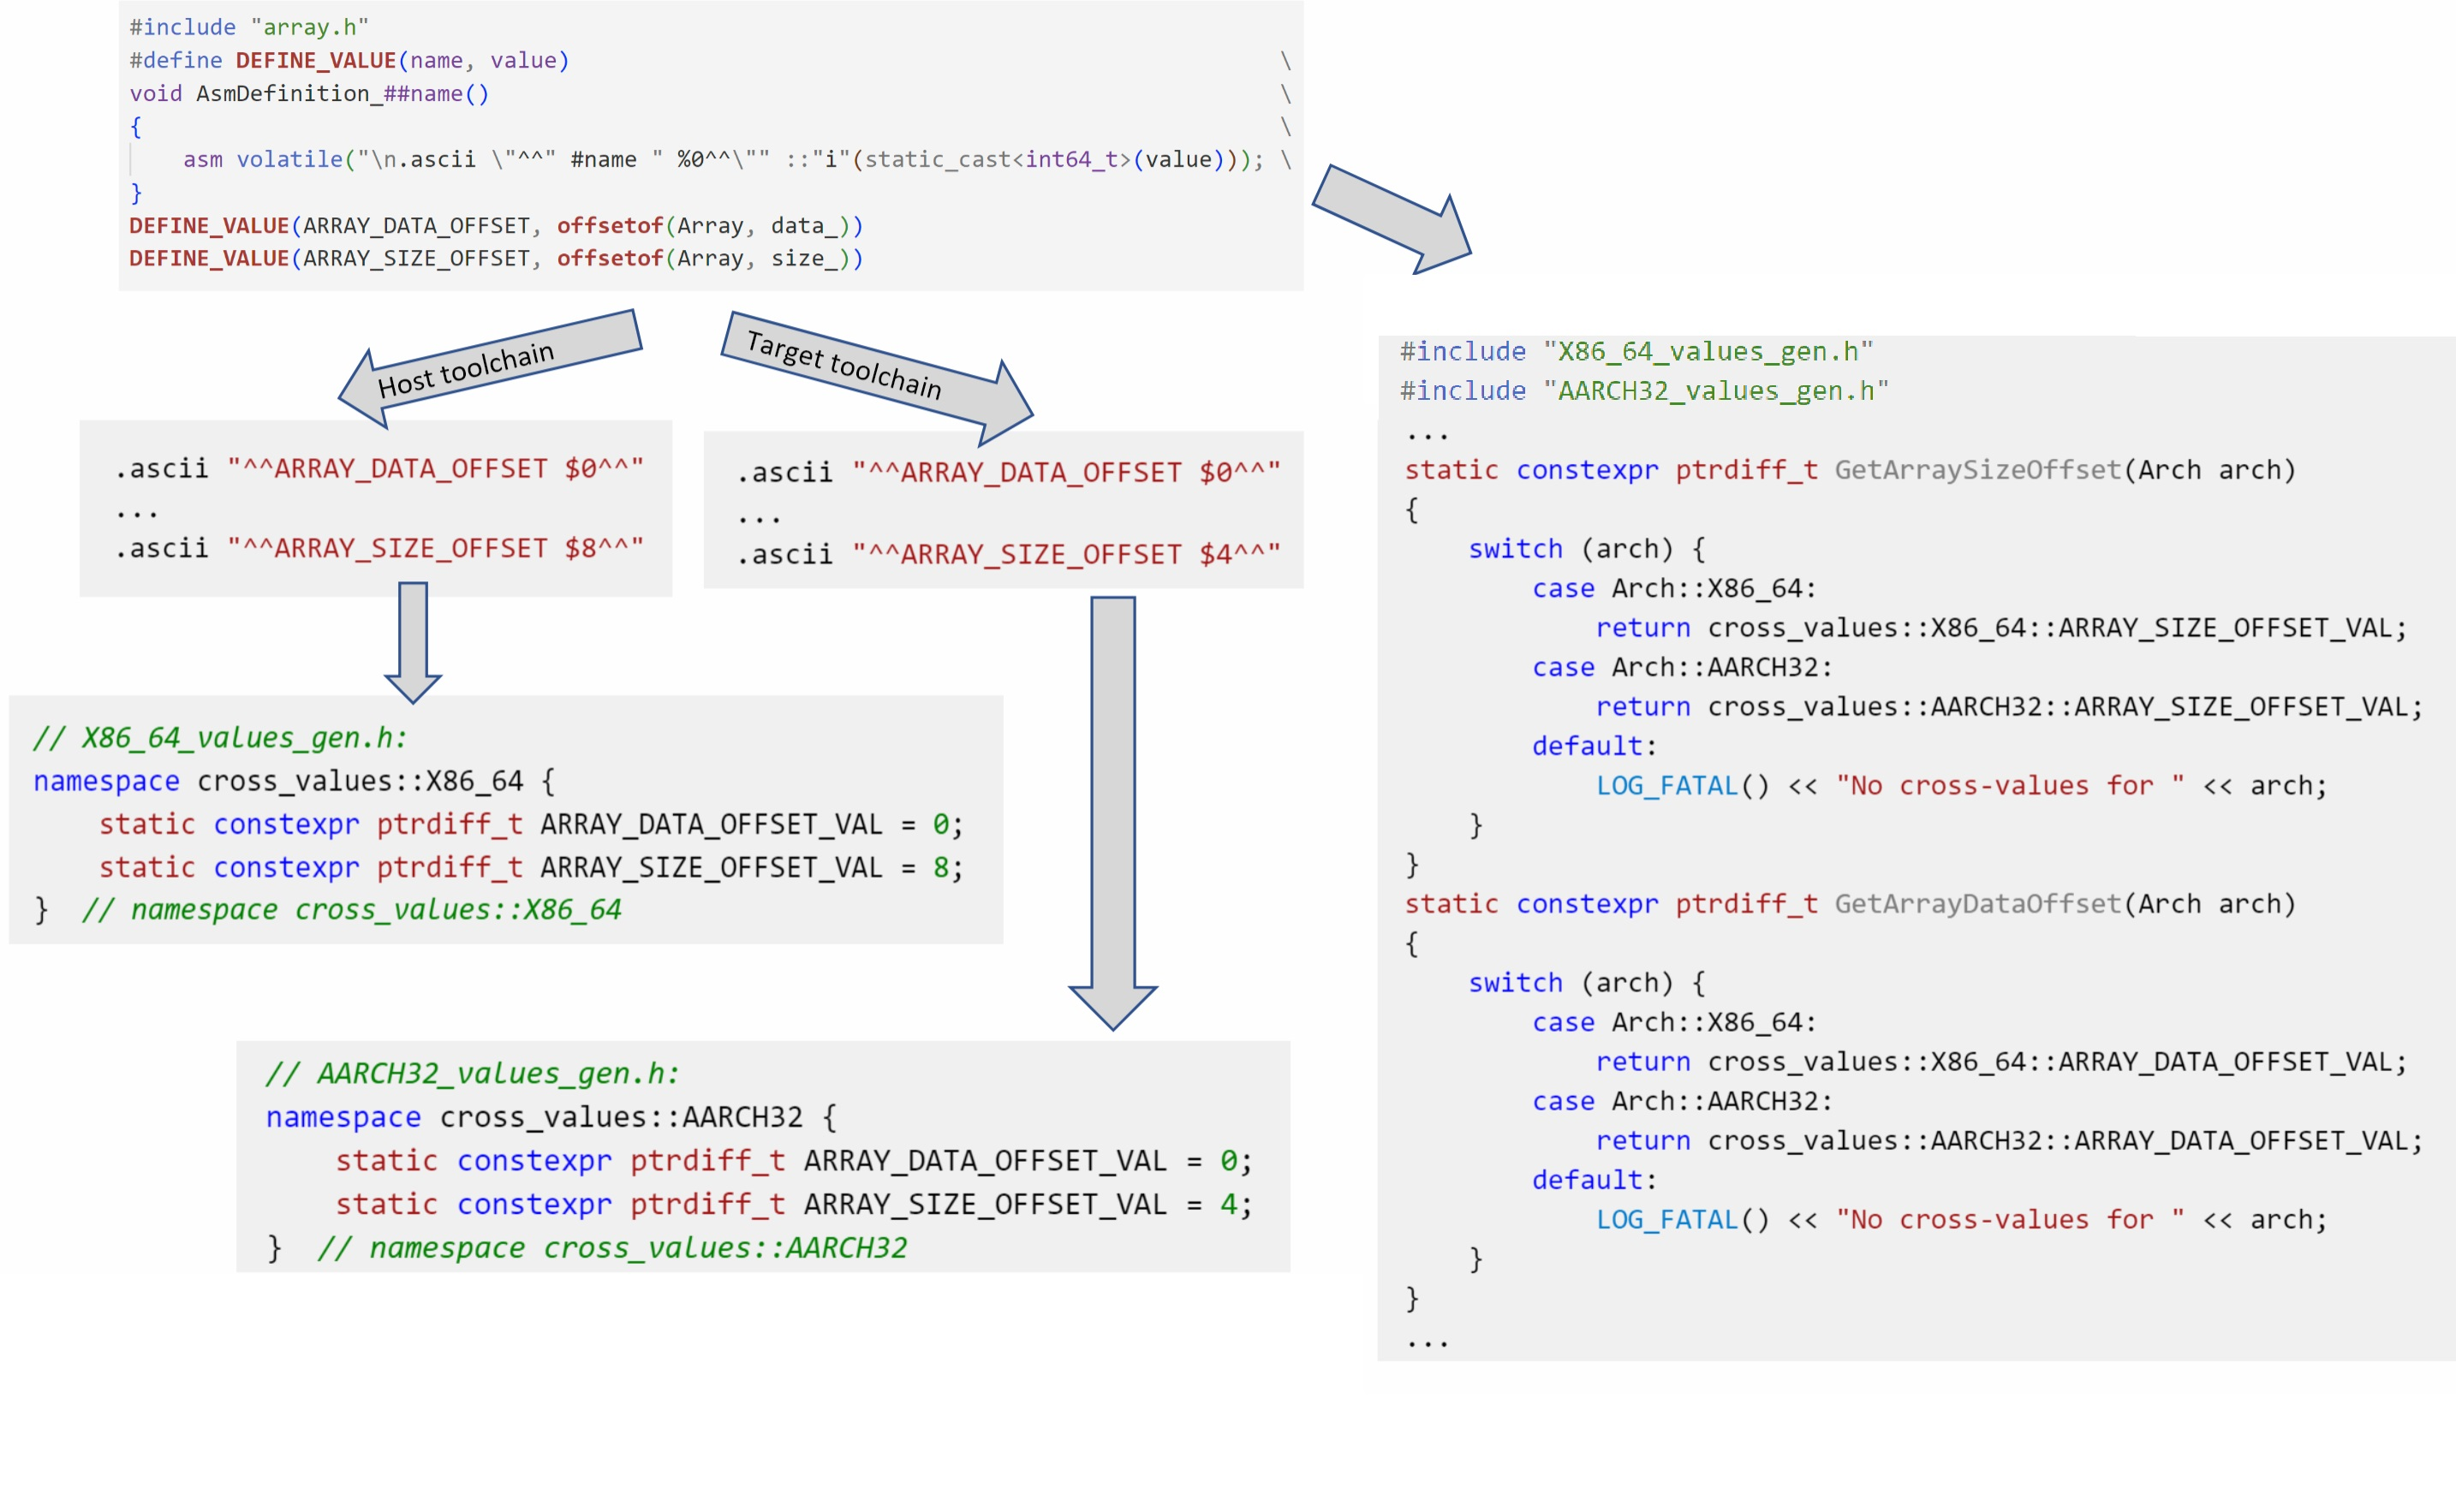
\includegraphics[scale=0.4]{asm_defines_getters.jpg}
    \caption{Схема генерации геттер-функций.}
    \label{fig:asm_defines_getters}
\end{figure}

Затем, конфигурация хост-сборки завершается и можно приступать к непосредственной сборке AOT-компилятора с помощью вызова утилиты Make \cite{make} или Ninja \cite{ninja}. Собранный таким образом компилятор располагает необходимыми значениями платформо-зависимых констант и способен генерировать корректный код для запуска в среде виртуальной машине, собранной тем же таргет-тулчейном, что и соответствующая вспомогательная директория.

\section{Детали и особенности реализации}
Основным принципом, соблюдаемым при разработке этого модуля являлось стремление к минимизации работы, связанной с его обслуживанием в будущем. В первую очередь это выражается в высоком уровне автоматизации процесса, описанного в предыдущей секции.

\par
Конфигурация вспомогательных директорий сборки происходит с использованием встроенного в \textit{CMake} модуля \textit{ExternalProject} \cite{cmake-ext-proj}.
Данный модуль позволяет встроить процессы скачивания, конфигурации, сборки и т.д. какого-то стороннего проекта в процесс сборки основного проекта, и предоставляя контроль за ними в терминах зависимостей и целей сборки.
Используя в качестве директории исходного кода стороннего проекта директорию, являющуюся деревом исходного кода для основной сборки виртуальной машины, а также указав соответствующий таргет-тулчейн образуются необходимые зависимости сборки для \textit{libasm\_defines.S} файлов (см. рис. \ref{fig:build_dir}), автоматически поддерживающие их консистентное состояние при модификациях в исходном коде.
В свою очередь, эти файлы являются входными для скриптов (см. ниже), осуществляющих генерацию файлов с определением констант в процессе сборки, а создание такой зависимости также влечёт консистентное состояние для них, в том числе. Тот факт, что они являются файлами-заголовками, позволяет построить необходимые зависимости к конечным целям сборки, включая AOT-компилятор. За счёт этого достигается корректность не только чистой сборки, но и инкрементальной, делая разработку виртуальной машины более удобной.

\par
Автоматизация обеспечивается не только с помощью \textit{CMake}, но и с помощью шаблонной генерации \textit{ERB} (сокращённо от \textit{Embedded Ruby}) \cite{erb}. Этот инструмент позволяет генерировать текстовые файлы любого формата, включая C++-код. Такой подход находит эффективное применение в обобщении однообразного кода, путём вынесения нетривиальной информации в один документ (например, \textit{JSON-} или \textit{YAML-}формата), а затем генерируя исходный код на основе его содержания по шаблону специального формата (\textit{.erb}-шаблон). К наиболее ярким его достоинствам относится явное выделение однообразия в коде (что упрощает его понимание и позволяет избежать многих ошибок, например из-за копирования кода), дешёвая с точки зрения разработки масштабируемость, возможность быстрого изменения функционала. В качестве основного документа, на основе которого производится весь описанный ранее процесс генерации, используется сама единица трансляции, изображённая на рисунке \ref{fig:asm_defines}, а также список \textit{cmake-toolchain} файлов, в том числе определяющий количество поддерживаемых AOT-компилятором платформ и сами платформы.

\par
Созданный C++-интерфейс представляет собой обычные C++-функции, имена которых основаны на именах соответствующих платформо-зависимых констант, принимающие в качестве аргумента переменную перечисляемого типа, отражающую выбранную платформу, и возвращающие значение константы на платформе согласно аргументу. Кроме того, сами константы доступны для использования непосредственно, так как находятся в отдельных пространствах имён. Это позволяет использовать данный модуль в как в платформо-определённых участках кода, так и обобщённых от платформы участках кода.

\section{Валидация}
На основе сгенерированных файлов с определениями констант вычисляется контрольная сумма.
В случае поддержки AOT-компилятором нескольких целевых платформ, контрольная сумма вычисляется для каждой из них, и соответствующее результату компиляции значение записывается в каждый выходной файл.
Аналогично, контрольная сумма записывается в образ самой виртуальной машины.
При инициализации AOT-файла происходит сравнение контрольной суммы, записанной в виртуальную машину и в AOT-файл. Это позволяет отследить ситуации расхождения констант и предотвратить ряд трудно обнаруживаемых ошибок.  

\newpage